% !TeX root = ../../../main.tex
\subsection{Results}
\label{ch08:sec:results}
\ChEightHeadingOnly


\subsubsection{\ChEightRebuttal{Structured EHR evidence calibrates event timing while preserving event recovery}}
\label{ch08:sec:main_results}

Table~\ref{ch08:tab:main_results_threshold_01} summarizes timeline reconstruction performance for text-only reconstruction and multimodal reconstruction with retrieved structured EHR evidence.
Across models, multimodal calibration has little effect on event match rate, indicating that structured rows do not primarily expand the set of events recovered from narrative text.
Instead, structured evidence primarily affects temporal localization, with effects that vary by model and metric.
These results support the role of structured rows as temporal evidence for text-derived events, rather than as a substitute event source.

\ChEightRebuttal{
Mean paired case-level temporal differences generally favored multimodal calibration: 4 of 6 models showed higher concordance and 3 of 6 showed higher AULTC, while no model showed lower performance on either temporal metric. However, uncertainty was substantial: no paired confidence interval for the multimodal--unimodal concordance difference excluded zero, and only DeepSeek V3.2 showed an AULTC interval entirely above zero ((\hyperref[ch08:supp:paired-bootstrap]{Supplementary Material \S\ref*{ch08:supp:paired-bootstrap}}, \hyperref[ch08:tab:supp-paired-bootstrap]{Table~\ref*{ch08:tab:supp-paired-bootstrap}})). Performance was generally higher on the i2b2-derived subset, but modality effects were source-dependent ((\hyperref[ch08:supp:dataset-stratified]{Supplementary Material \S\ref*{ch08:supp:dataset-stratified}}, Tables~\hyperref[ch08:tab:supp-i2b2]{\ref*{ch08:tab:supp-i2b2}}--\hyperref[ch08:tab:supp-mimiciv]{\ref*{ch08:tab:supp-mimiciv}})).}

Because event match rate depends on the semantic matching threshold used to align predicted and reference events, we also vary the event-matching threshold and examine the relationship between event recovery and temporal quality.
Figure~\ref{ch08:fig:threshold_sweeps_main} shows AULTC and concordance as functions of event match rate across thresholds.
Across operating points, multimodal reconstruction generally occupies a similar event-recovery range as text-only reconstruction while changing temporal performance, especially AULTC, for several models.
This supports the same broad conclusion as Table~\ref{ch08:tab:main_results_threshold_01}: retrieved structured rows primarily affect temporal calibration rather than event discovery.



% !TeX root = ../../../main.tex
\begin{table}[htbp]
\caption{Performance on 40 discharge summaries at event-matching threshold $0.1$ for unimodal and multimodal timeline reconstruction. Values are point estimates with bootstrap 95\% confidence intervals in brackets. \textbf{Bold} indicates the best point estimate within each metric--modality column.}\ChEightFloatLabel{ch08:tab:main_results_threshold_01}
\ChEightTableBodyStart
\begin{ChEightFloatBody}

{\footnotesize
\setlength{\tabcolsep}{3pt}
\renewcommand{\arraystretch}{1.12}

\begin{adjustbox}{max width=\textwidth}
\begin{tabular}{lcccccc}
\hline
\multirow{2}{*}{\textbf{Model}} 
& \multicolumn{2}{c}{\textbf{Event match rate}} 
& \multicolumn{2}{c}{\textbf{Concordance}} 
& \multicolumn{2}{c}{\textbf{AULTC}} \\
\cline{2-7}
& \textbf{Unimodal} & \textbf{Multimodal} 
& \textbf{Unimodal} & \textbf{Multimodal} 
& \textbf{Unimodal} & \textbf{Multimodal} \\
\hline
DeepSeek R1
& 0.39 [0.32, 0.47]
& 0.39 [0.32, 0.47]
& 0.75 [0.69, 0.79]
& 0.75 [0.70, 0.80]
& \textbf{0.80 [0.76, 0.82]} 
& \textbf{0.79 [0.77, 0.82]}\\

KimiK2-Instruct
& 0.26 [0.21, 0.29]
& 0.25 [0.22, 0.30]
& 0.73 [0.69, 0.76]
& 0.74 [0.68, 0.81]
& 0.68 [0.61, 0.73]
& 0.68 [0.62, 0.73] \\

GPT-OSS-120B
& 0.32 [0.27, 0.37]
& 0.32 [0.28, 0.37]
& 0.74 [0.70, 0.77]
& 0.75 [0.71, 0.80]
& 0.76 [0.72, 0.80] 
& 0.77 [0.74, 0.81]\\

DeepSeek V3.2
& \textbf{0.49 [0.43, 0.56]}
& \textbf{0.49 [0.43, 0.56]}
& 0.74 [0.70, 0.80]
& 0.77 [0.73, 0.81]
& 0.71 [0.64, 0.78] 
& 0.77 [0.73, 0.81]\\

GLM5
& 0.33 [0.27, 0.39]
& 0.33 [0.27, 0.40]
& \textbf{0.80 [0.78, 0.83]}
& \textbf{0.82 [0.75, 0.84]}
& 0.78 [0.73, 0.82] 
& 0.78 [0.73, 0.82]\\

Qwen3.5-397B-A17B
& 0.38 [0.28, 0.47]
& 0.40 [0.29, 0.51]
& 0.78 [0.72, 0.81]
& 0.79 [0.78, 0.82]
& 0.74 [0.68, 0.77] 
& 0.77 [0.74, 0.78]\\

\hline
\end{tabular}
\end{adjustbox}


}


\end{ChEightFloatBody}
\end{table}



% !TeX root = ../../../main.tex
\begin{figure}[htbp]
\begin{ChEightFloatBody}

    \centering
    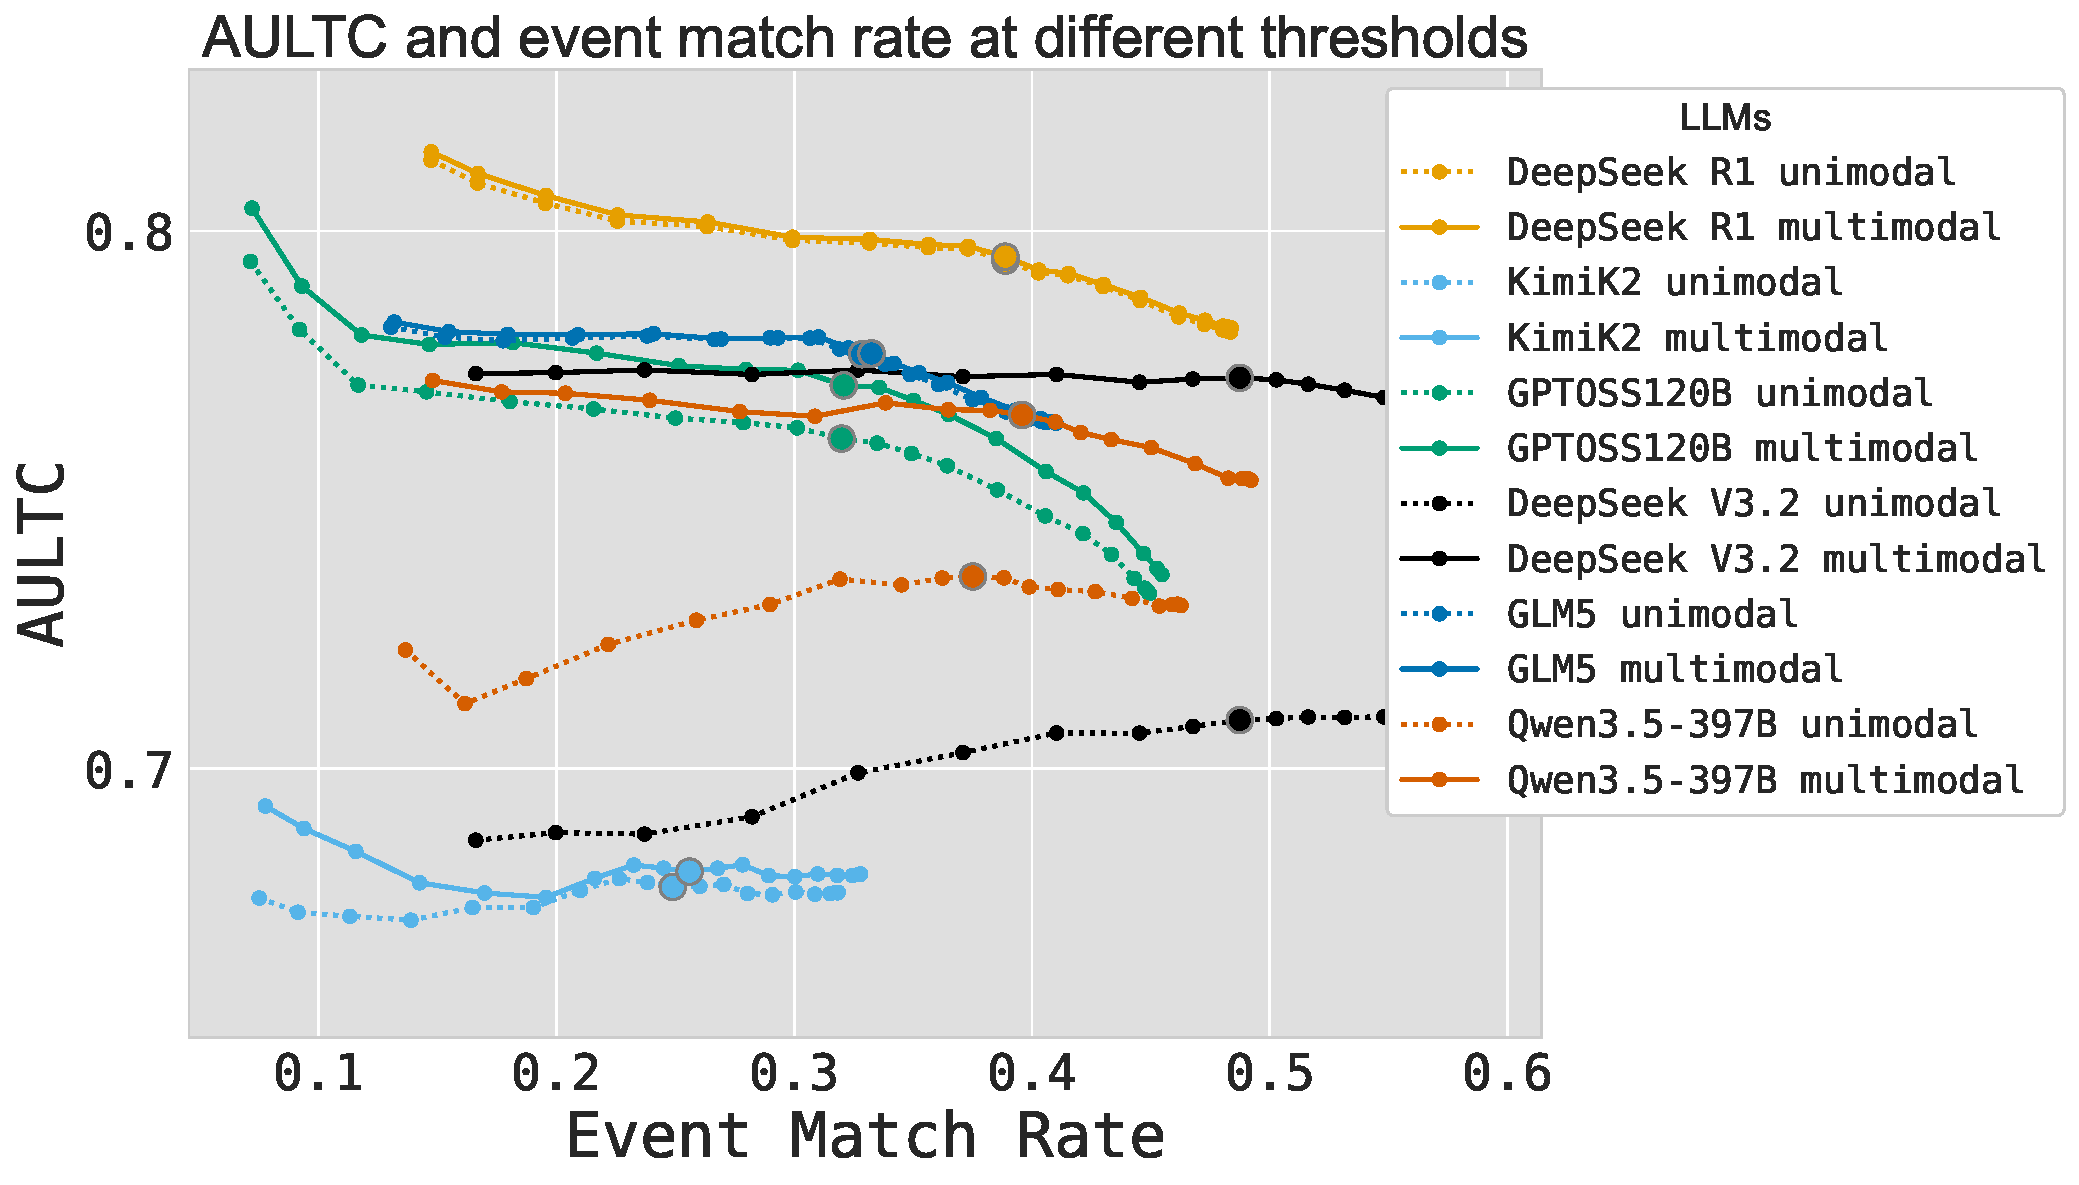
\includegraphics[width=0.479\textwidth]{Chapters/chapter-08/images/plots/aultc_vs_emr_n40_v2.pdf}
    \hfill
    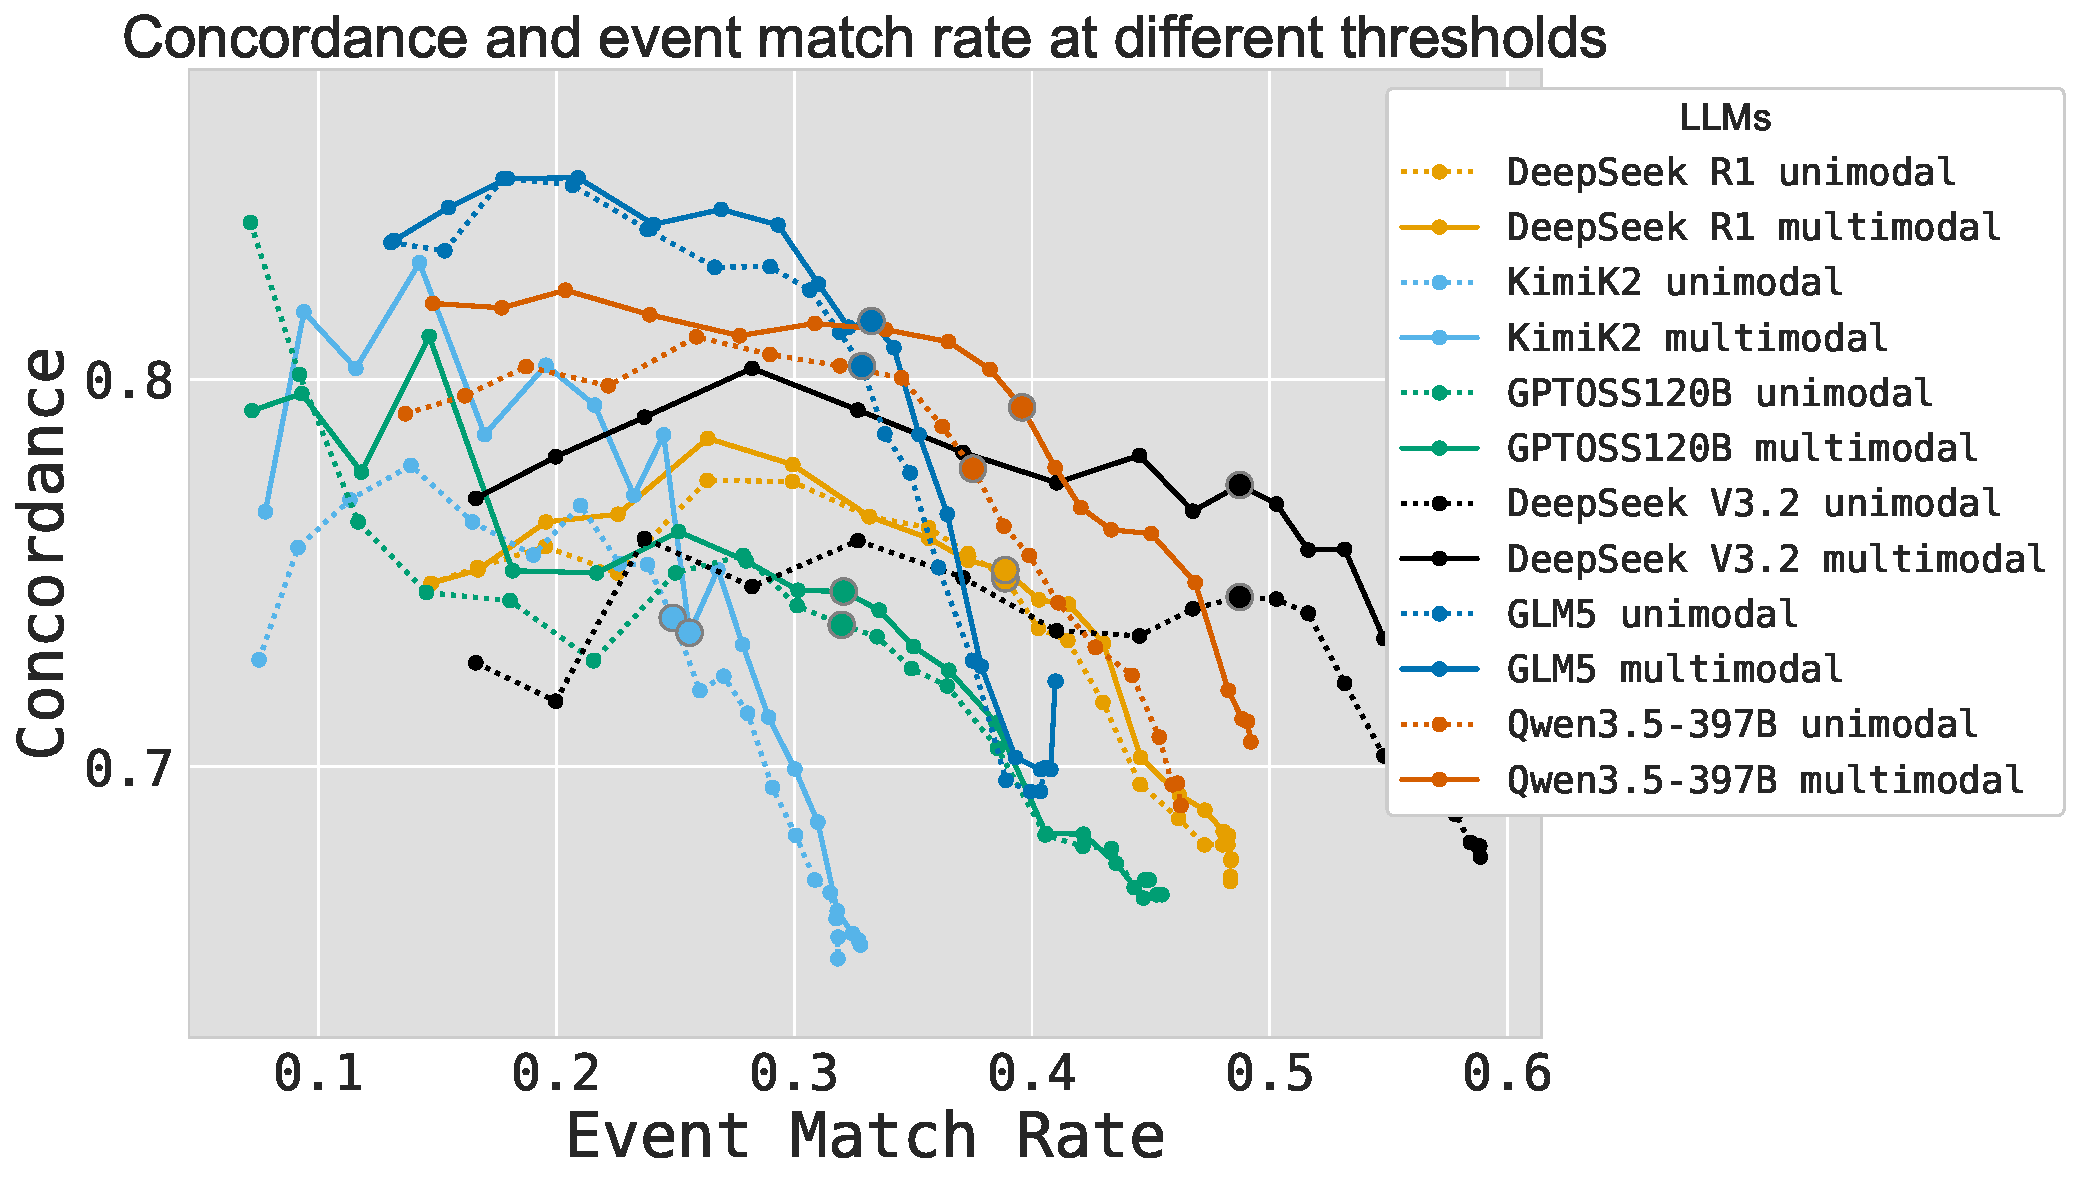
\includegraphics[width=0.479\textwidth]{Chapters/chapter-08/images/plots/cidx_vs_emr_n40_v2.pdf}

    
    \begin{minipage}[t]{0.485\textwidth}
        \centering
    \end{minipage}
    \hfill
    \begin{minipage}[t]{0.485\textwidth}
        \centering
    \end{minipage}

    
    
    
    

\end{ChEightFloatBody}
\caption{Temporal performance versus event match rate across event-matching thresholds for unimodal and multimodal variants of each model on the 40-summary evaluation set. (\textbf{Left}) AULTC versus event match rate. (\textbf{Right}) Temporal concordance versus event match rate.}\ChEightFloatLabel{ch08:fig:threshold_sweeps_main}
\end{figure}




\noindent\textbf{Scaffold ablations.}
Table~\ref{ch08:tab:ablation_and_DTW}A evaluates whether the staged scaffolded workflow is necessary, or whether similar performance can be obtained by generating a complete timeline in one step with retrieved structured rows.
The single-step formulation performs worse than the full scaffolded variant, suggesting that clinical timeline reconstruction benefits from first identifying temporally informative anchor events before reconstructing the full event set.
The stage at which structured evidence is introduced also matters.
Final-stage calibration yields the highest event match rate, but the strongest temporal metrics are obtained when structured evidence is used both to calibrate the anchor scaffold and to refine the final assembled timeline.
This supports the design choice of using structured rows first to stabilize the temporal backbone of the encounter and then to recalibrate the expanded trajectory.


% !TeX root = ../../../main.tex
\begin{table}[htbp]
\caption{\ChEightRebuttal{\textbf{(A)} DeepSeek V3.2 scaffold and calibration-stage ablations with bootstrap 95\% confidence intervals. \textbf{(B)} Retrieval calibration compared with sentence-embedding and lexical Dynamic Time Warping (DTW) alignments.}}\ChEightFloatLabel{ch08:tab:ablation_and_DTW}
\ChEightTableBodyStart
\begin{ChEightFloatBody}
 
\setlength{\tabcolsep}{3pt} \renewcommand{\arraystretch}{1.08} 
 
\begin{minipage}{\textwidth} 
\scriptsize 
\noindent\textbf{A. Scaffold and calibration-stage ablations}\par

\begin{adjustbox}{max width=\linewidth}
\begin{tabular}{@{\extracolsep{\fill}}lcccccc@{}} 
\hline 
\multirow{2}{*}{\textbf{Ablation}} 
& \multicolumn{2}{c}{\textbf{Event match rate}} 
& \multicolumn{2}{c}{\textbf{Concordance}} 
& \multicolumn{2}{c}{\textbf{AULTC}} \\ 
\cline{2-7} 
& \textbf{Unimodal} 
& \textbf{Multimodal} 
& \textbf{Unimodal} 
& \textbf{Multimodal} 
& \textbf{Unimodal} 
& \textbf{Multimodal} \\ 
\hline 
single-step 
& 0.39 [0.35, 0.45] 
& 0.39 [0.35, 0.44] 
& 0.70 [0.65, 0.74] 
& 0.71 [0.65, 0.75] 
& \textbf{0.78 [0.74, 0.83]} 
& \textbf{0.77 [0.73, 0.83]} \\ 
central only 
& -- 
& 0.46 [0.42, 0.51] 
& -- 
& 0.72 [0.66, 0.77] 
& -- 
& 0.75 [0.71, 0.80] \\ 
final only 
& \textbf{0.51 [0.46, 0.56]} 
& \textbf{0.52 [0.46, 0.58]} 
& 0.68 [0.64, 0.72] 
& 0.69 [0.64, 0.72] 
& 0.72 [0.67, 0.78] 
& 0.73 [0.69, 0.78] \\ 
central + final 
& 0.49 [0.43, 0.56]
& 0.49 [0.43, 0.56]
& \textbf{0.74 [0.70, 0.80]}
& \textbf{0.77 [0.73, 0.81]}
& 0.71 [0.64, 0.78] 
& \textbf{0.77 [0.73, 0.81]} \\
\hline 
\end{tabular}
\end{adjustbox}


\noindent\textit{Note:} Central-only, final-only, and central + final correspond to updating the anchor scaffold only, the final timeline only, or both stages, respectively. The central-only condition yields a single final timeline and is undefined for the unimodal setting.


\noindent\textbf{B. Retrieval calibration vs. explicit temporal alignment (Dynamic Time Warping)}


\begin{adjustbox}{max width=\textwidth}
\begin{tabular}{@{}l*{9}{c}@{}}
\hline
\multirow{2}{*}{\textbf{Model}}
& \multicolumn{3}{c}{\textbf{Event match rate}}
& \multicolumn{3}{c}{\textbf{Concordance}}
& \multicolumn{3}{c}{\textbf{AULTC}} \\
\cline{2-4}\cline{5-7}\cline{8-10}
& \textbf{Retrieval}
& \textbf{DTW(Sent)}
& \textbf{DTW(Lex)}
& \textbf{Retrieval}
& \textbf{DTW(Sent)}
& \textbf{DTW(Lex)}
& \textbf{Retrieval}
& \textbf{DTW(Sent)}
& \textbf{DTW(Lex)} \\
\hline
DeepSeek R1
& 0.39 & 0.39 & 0.39
& 0.75 & 0.75 & 0.74
& 0.79 & 0.80 & 0.79 \\

KimiK2-Instruct
& 0.25 & 0.26 & 0.26
& 0.74 & 0.74 & 0.73
& 0.68 & 0.68 & 0.68 \\

GPT-OSS-120B
& 0.32 & 0.32 & 0.32
& 0.75 & 0.73 & 0.73
& 0.77 & 0.77 & 0.77 \\

DeepSeek V3.2
& 0.49 & 0.49 & 0.49
& 0.77 & 0.76 & 0.77
& 0.77 & 0.77 & 0.77 \\

GLM5
& 0.33 & 0.33 & 0.33
& 0.82 & 0.81 & 0.81
& 0.78 & 0.78 & 0.77 \\

Qwen3.5-397B-A17B
& 0.40 & 0.40 & 0.40
& 0.79 & 0.79 & 0.79
& 0.77 & 0.77 & 0.77 \\
\hline
\end{tabular}
\end{adjustbox}



\end{minipage}




\end{ChEightFloatBody}
\end{table}


\noindent\textbf{Explicit temporal alignment.}
We also compare retrieval-based calibration with dynamic time warping (DTW), an explicit temporal-alignment baseline that aligns text-derived events with structured rows as sequences (Table~\ref{ch08:tab:ablation_and_DTW}B).
The two approaches achieve broadly comparable accuracy: DTW is slightly higher for some model--metric pairs, while retrieval-based calibration is slightly higher for others, and the differences are small relative to the variability reflected by the bootstrap confidence intervals in Table~\ref{ch08:tab:main_results_threshold_01}.  \ChEightRebuttal{Retrieval and DTW therefore show comparable aggregate accuracy rather than quantitative superiority. Their principal distinction is structural: retrieval presents event-specific candidates and can retain a text-derived estimate when no adequate counterpart exists, whereas DTW imposes monotone sequence alignment across modalities with incomplete and asymmetric event coverage.}



\subsubsection{\ChEightRebuttal{Complementary coverage of narrative and structured records}}
\label{ch08:sec:gap_results}


The main reconstruction results show that structured rows can improve event timing when used as calibration evidence.
We next ask why structured records cannot simply replace narrative text and then
\ChEightRebuttal{characterize which narrative-derived events are poorly represented in structured EHR data; because this text-to-structure analysis does not assess structured-only events, it supports complementarity rather than completeness of either modality. We compare text-derived timelines against tabular records from the same encounters. }
The analysis uses the best-performing LLM-generated event timelines as the textual view, MIMIC structured data as the tabular view, and admission or the case reference time as the shared temporal anchor.
For each text-derived event, we retrieve a candidate tabular counterpart using embedding-based similarity matching and evaluate it along two dimensions: semantic adequacy and temporal alignment.
Semantic adequacy is assessed using retrieval-augmented scoring on a 0--1 scale, while temporal alignment is measured as the absolute difference in hours between the text-derived timestamp and the matched tabular timestamp.
Based on these criteria, each event is classified as \textbf{well captured}, \textbf{complete absence}, \textbf{temporal mismatch}, \textbf{semantic distance}, or \textbf{detail gap}.
Table~\ref{ch08:tab:gap_analysis} summarizes the distribution of these categories.


% !TeX root = ../../../main.tex
\begin{table}[htbp]
\caption{Structured-data gap analysis. Each text-derived event is compared with structured EHR counterparts from the same encounter.}\ChEightFloatLabel{ch08:tab:gap_analysis}
\ChEightTableBodyStart
\begin{ChEightFloatBody}

{
\setlength{\tabcolsep}{5pt}
\renewcommand{\arraystretch}{1.12}

\begin{adjustbox}{max width=0.9\textwidth}
\scriptsize
\begin{tabular}
{>{\raggedright\arraybackslash}p{0.15\textwidth}>{\raggedright\arraybackslash}p{0.65\textwidth}>{\raggedright\arraybackslash}p{0.16\textwidth}}
\hline
\textbf{Category} & \textbf{Definition} & \textbf{Count (\%)} \\
\hline
Well captured 
& Semantically adequate structured counterpart within the temporal window 
& 2,827 (33.5\%) \\

Complete absence 
& No structured counterpart identified 
& 2,963 (35.1\%) \\

Temporal mismatch 
& Semantically related structured row exists but occurs outside the temporal window 
& 1,463 (17.3\%) \\

Semantic distance 
& Retrieved row is not clinically equivalent to the narrative event 
& 801 (9.5\%) \\

Detail gap 
& Structured row omits clinically important attributes such as severity, laterality, duration, progression, or functional status 
& 385 (4.6\%) \\
\hline
Total textual events & -- & 8,439 \\
\hline
\end{tabular}
\end{adjustbox}


}


\end{ChEightFloatBody}
\end{table}
















Across 8,439 text-derived events, only 33.5\% are well captured by structured data, while 35.1\% have no structured counterpart at all.
When a structured counterpart exists, its timestamp is often useful: the median temporal discrepancy is 4.3 hours, with 58.4\% of matched events within 6 hours, 69.5\% within 12 hours, and 79.3\% within 24 hours.
The missing events are not merely low-value narrative detail; they include symptoms, functional status, temporal qualifiers, patient-reported information, severity descriptions, and clinical context.
Representative complete-absence examples include \textbf{symptom descriptions} such as ``substernal chest pain for 1 day'' and ``developed chest pain''; \textbf{denial statements} such as ``no seizure-like activity'' and ``no deformity''; \textbf{temporal patterns} such as ``pain resolved'' and ``improving clots on LE''; \textbf{severity descriptors} such as ``EF 55\%'' and ``non-small cell lung cancer stage IIIA''; and \textbf{causal or procedural context} such as ``intubated for several days after second surgery'' and ``repair of leak from pouch.''
These findings explain why structured rows are useful for temporal calibration but incomplete as representations of patient trajectories.


\subsubsection{Qualitative case study: text supplies phenotype, tables calibrate time}
\label{ch08:sec:vignette_results}


Figure~\ref{ch08:fig:motivation_multimodal_alignment} illustrates the qualitative behavior of the pipeline using a synthetic stroke-alert case.
The narrative supplies clinically decisive phenotype details, including lobar hemorrhage location, hematoma volume, aphasia, plegia, command following, absence of intraventricular hemorrhage or hydrocephalus, and repeat-CT stability.
The structured rows provide sparse but precise temporal anchors, including admission time and IV andexanet alfa administration.
The text-only scaffold recovers the reversal event but places it shortly after the initial CT at approximately \(+1.5\)h; retrieval-augmented calibration links the event to the medication-administration row and shifts reversal to \(+6.5\)h relative to admission.

\begin{tcolorbox}[
    breakable,
    colback=white,
    colframe=black!45,
    title=\textbf{Pipeline output: calibrated event timeline},
    fonttitle={\fontsize{8pt}{11pt}\selectfont\bfseries}
]
\scriptsize
\setlength{\parindent}{0pt}

\newcommand{\ChEightVignetteRow}[3]{%
\noindent
\begin{minipage}[t]{0.47\linewidth}\raggedright #1\end{minipage}\hfill
\begin{minipage}[t]{0.10\linewidth}\raggedleft #2\end{minipage}\hfill
\begin{minipage}[t]{0.37\linewidth}\raggedright #3\end{minipage}\par\vspace{1.5pt}
}



\noindent
\begin{minipage}[t]{0.47\linewidth}\raggedright \textbf{Event}\end{minipage}\hfill
\begin{minipage}[t]{0.10\linewidth}\raggedleft \textbf{Time (h)}\end{minipage}\hfill
\begin{minipage}[t]{0.37\linewidth}\raggedright \textbf{Source / calibration note}\end{minipage}

\vspace{2pt}
\hrule
\vspace{3pt}
\ChEightVignetteRow{Last known well at 0730}{-5.5}{Text clock time relative to admission}
\ChEightVignetteRow{Found down at home}{-1.0}{Text-derived estimate}
\ChEightVignetteRow{67 years old}{0.0}{Text, admission context}
\ChEightVignetteRow{Atrial fibrillation}{0.0}{Text, admission context}
\ChEightVignetteRow{Admitted/brought in as stroke alert}{0.0}{\textbf{Table}, anchored by admission row at 1300}
\ChEightVignetteRow{Dense right arm plegia}{0.0}{Text, anchored to admission}
\ChEightVignetteRow{Follows commands}{0.0}{Text, anchored to admission}
\ChEightVignetteRow{Initial CT showed intracerebral hemorrhage}{0.5}{Text-derived estimate}
\ChEightVignetteRow{Estimated hematoma volume $\sim$55 mL}{0.5}{Text, anchored to initial CT}
\ChEightVignetteRow{Left frontal lobar location of hemorrhage}{0.5}{Text, anchored to initial CT}
\ChEightVignetteRow{Reversal agent was administered}{6.5}{\textbf{Table}, corrected by IV andexanet alfa at 1930}
\ChEightVignetteRow{Repeat CT was stable}{8.5}{Text, inferred sequentially post-reversal}

% 
\hrule
\end{tcolorbox}


















\textbf{}This case illustrates the asymmetry motivating the workflow. Text is necessary to recover clinically meaningful phenotype information, while structured rows calibrate selected time-sensitive events when relevant counterparts exist. The resulting trajectory could support human-reviewed cohort definition or eligibility logic by preserving narrative-only clinical details while grounding treatment timing in structured evidence. 
For example, the 2024 ENRICH trial comparing surgical evacuation versus medical management had eligibility criteria beyond what would be available in structured data alone\cite{pradilla2024trial}. 
Structured data could show admission indication (hemorrhagic stroke), medication events (a confirmation proxy), and functional status scores (neurologic and disability level), but the notes contain key additional ENRICH eligibility features and timing: 55 mL hematoma volume ($30<x<80$), left frontal lobar location (lobar/anterior basal ganglionic), aphasia/plegia (new onset of neurological symptoms), no IVH/hydrocephalus and stable repeat imaging (feasibility), as well as localization of the eligibility timing window (within 24 hours of last known well time).


